\documentclass[12pt]{article}

\usepackage{sbc-template}
\usepackage{graphicx,url}
\usepackage[utf8]{inputenc}
\usepackage[brazilian]{babel}
\usepackage{booktabs}
\usepackage{multirow}
\usepackage{amsmath}
\usepackage{longtable}
\usepackage{array}
\usepackage{xcolor}

% Comando para destacar seções ainda a preencher
\newcommand{\TODO}[1]{\textcolor{red}{[TODO: #1]}}

\sloppy

\title{Análise de Gravidade de Sinistros \\ 
nas Rodovias Federais Brasileiras}

\author{
  Davi da Silva Romão\inst{1},
  Diogo Tallys da Mota Amorim\inst{1},\\
  Gabriel Gomes de Oliveira\inst{1},
  Thiago Ribeiro da Silva\inst{1}
}

\address{
  Instituto de Computação -- Universidade Federal de Alagoas (UFAL)\\
  Maceió -- AL -- Brasil
  \email{\{dsr,dtma,ggo,trs\}@ic.ufal.br}
}

\begin{document}

\maketitle

% ============================================================
\begin{abstract}
This work analyzes 300,086 records of traffic accidents on Brazilian
federal highways between 2022 and 2026, aiming to identify the
combinations of temporal, spatial, causal, and infrastructural factors
associated with accident severity. After data cleaning and feature
engineering, bivariate association tests, odds ratio analysis, STL
time-series decomposition, and spatial concentration analysis via the
Lorenz curve were applied to verify five hypotheses. Results show that
accident type is the strongest individual predictor of fatality
(Cramér's V = 0.344); roundabouts present the highest protective
effect among road geometry attributes (OR = 0.287); weekend trips
increase fatal proportions regardless of traffic volume
(RR = 1.256); 13.9\% of the road network concentrates 50\% of
fatal incidents; and regional fatality rates are significantly associated with single-lane road density ($\chi^2 = 2023.65$, $p < 0.001$), with North and Northeast regions exhibiting twice the fatality rate of South and Southeast regions.
The findings provide quantitative support for resource allocation
decisions by road safety agencies.
\end{abstract}

\begin{resumo}
Este trabalho analisa 300.086 registros de sinistros de trânsito
ocorridos nas rodovias federais brasileiras entre 2022 e 2026, com o
objetivo de identificar combinações de fatores temporais, espaciais,
causais e infraestruturais associadas à gravidade das ocorrências.
Após limpeza e engenharia de \textit{features}, aplicamos testes
de associação bivariada, análise de razão de chances, decomposição STL
e análise de concentração espacial via curva de Lorenz para verificar
cinco hipóteses. Os resultados mostram que o tipo de acidente é o
preditor individual mais relevante (V de Cramér = 0,344); rotatórias
apresentam o maior efeito protetor entre os atributos de traçado
(OR = 0,287); fins de semana elevam a proporção fatal independentemente
do volume de tráfego (RR = 1,256); 13,9\% da malha concentra 50\%
dos fatais; e as taxas de fatalidade regionais estão significativamente associadas à densidade de pistas simples ($\chi^2 = 2023,65$, $p < 0,001$), com as regiões Norte e Nordeste registrando taxas de fatalidade duas vezes superiores às das regiões Sul e Sudeste.
Os achados fornecem suporte quantitativo para decisões de alocação
de recursos por órgãos de segurança viária.
\end{resumo}

% ============================================================

\newpage

% ============================================================
\section{Introdução}
% ============================================================

Todo ano, os acidentes em rodovias federais brasileiras consomem
recursos de saúde, reduzem a produtividade e deixam sequelas
permanentes em famílias. Diante desse cenário, a Polícia Rodoviária
Federal (PRF) e o Departamento Nacional de Infraestrutura de
Transportes (DNIT) precisam decidir onde, quando e como atuar.
Este trabalho examina 300.086 registros de sinistros entre 2022 e
2026 para identificar quais combinações de fatores temporais,
espaciais, meteorológicos, causais e infraestruturais elevam a
probabilidade de morte. O objetivo é subsidiar três decisões
práticas: alocação de efetivo, priorização de obras e
dimensionamento de resposta emergencial.

As hipóteses investigadas são:

\begin{description}
  \item[H1] Causas comportamentais (ingestão de álcool, uso de
    substâncias psicoativas e sono ao volante) ocorrem com maior
    frequência no período noturno e estão associadas a maior
    gravidade do sinistro em comparação com outras causas no
    mesmo horário.

  \item[H2] Fins de semana, feriados e períodos de férias concentram
    maior frequência absoluta e maior proporção de sinistros com
    vítimas fatais, refletindo padrões de tráfego intenso e
    comportamento de risco.

  \item[H3] Condições meteorológicas adversas têm impacto
    diferenciado sobre a gravidade dos sinistros dependendo da
    região do país.

  \item[H4] A distribuição dos sinistros não é uniforme: trechos
    específicos de rodovias concentram parcela desproporcional
    das ocorrências fatais.

  \item[H5] O perfil de gravidade dos sinistros difere entre as
    cinco regiões brasileiras, com regiões de maior extensão de
    pista simples apresentando taxas de fatalidade superiores
    às de maior infraestrutura duplicada.
\end{description}


% ============================================================
\section{Base de Dados}
% ============================================================

\subsection{Descrição da Base}

A base utilizada é o conjunto de dados de sinistros de trânsito
agrupados por ocorrência, disponibilizado publicamente pela Polícia
Rodoviária Federal (PRF) no Portal de Dados Abertos do Governo
Federal~\cite{prf:2024}. Os registros derivam do Boletim de Acidente
de Trânsito (BAT), com atualização mensal e série histórica desde
2007. O recorte temporal adotado compreende os anos de 2022 a 2026;
o limite inferior foi definido para eliminar o viés pandêmico de 2020
e 2021, período em que a redução artificial do volume de tráfego
distorce análises de tendência e sazonalidade. Com esse recorte, a
base bruta totaliza \textbf{301.532 registros}, organizados em cinco
dimensões principais: variáveis temporais (data, horário, dia da
semana), espaciais (UF, município, rodovia, quilometragem e
coordenadas geográficas), causais (causa e tipo de acidente e
classificação de gravidade), infraestruturais (condição
meteorológica, tipo e traçado da pista, uso do solo) e de
consequências (mortos, feridos leves, feridos graves e ilesos).

% ============================================================
\subsection{Análise Estrutural e Limpeza dos Dados}

A base bruta passou por um processo de limpeza estruturado em cinco etapas: (i) remoção das colunas \texttt{regional}, \texttt{delegacia} e \texttt{uop}, que contêm metadados administrativos internos com inconsistências geográficas; (ii) exclusão da coluna \texttt{id} e de 6 registros duplicados por ela mascarados; (iii) correção da tipagem das variáveis \texttt{km}, \texttt{latitude} e \texttt{longitude} (strings com vírgula convertidas para float) e correção ortográfica de \texttt{condicao\_metereologica}; (iv) exclusão de 5 registros nulos em \texttt{classificacao\_acidente} (análise de sensibilidade indicou impacto máximo de 0,0017 p.p., inferior ao erro padrão SE = 0,055 p.p.); e (v) remoção de 1.435 registros com \texttt{km = 0} (756 registros anômalos com \texttt{br = 0} e \texttt{sentido\_via} nulo, validados por IC de Wilson 95\% \cite{wilson:1927}, e 679 registros violando a especificação posicional mínima da PRF de 0,1 km \cite{prf:dicionario}, cuja imputação geraria ruído espacial). Após a limpeza, a base resultante totalizou \textbf{300.086 registros}.

% ============================================================
\subsection{Engenharia de Features}

A partir da base limpa, foram criadas variáveis para enriquecer
a representação temporal, espacial e causal dos sinistros.

As colunas \texttt{data\_inversa} e \texttt{horario} foram combinadas
em \texttt{data\_hora}, a partir da qual se extraíram faixas horárias
(madrugada, manhã, tarde, noite), mês, estação do ano (hemisfério sul),
e indicadores binários de fim de semana e feriado nacional — incluindo
feriados móveis (Carnaval, Sexta-Feira Santa, Corpus Christi) calculados
via data da Páscoa. A variável \texttt{tracado\_via}, que armazenava
múltiplas características separadas por ponto e vírgula, foi decomposta
em 12 binárias independentes por codificação \textit{multilabel}.

A variável \texttt{causa\_acidente} apresentava 76 categorias, das quais
76,3\% representavam individualmente menos de 1\% dos registros,
caracterizando distribuição altamente esparsa. As causas foram
consolidadas em 8 grupos por similaridade semântica observada:
falha de atenção e reação, infração e comportamento de risco, falha
mecânica, infraestrutura e sinalização, condição ambiental, obstrução
da via, condição de saúde do condutor e envolvimento de pedestre.
Após a consolidação, nenhum grupo ficou abaixo de 0,5\% dos registros.

A variável \texttt{km} foi discretizada em faixas de 5 km. A comparação
entre tamanhos de \textit{bucket} revelou retornos decrescentes: a
transição de 1 para 5 km ganha 6,1 p.p.\ na proporção de intervalos
com suporte adequado ($\geq$ 30 registros), enquanto os passos
seguintes rendem apenas 3,6 e 1,8 p.p.\ a custo de metade da
resolução espacial. O bucket de 5 km representa o ponto de inflexão,
resultando em 254 intervalos com 82,3\% de cobertura adequada.
Por fim, \texttt{uf} foi mapeada para região geográfica brasileira.
O conjunto completo está descrito na Tabela~\ref{tab:features}.

\begin{table}[ht]
\centering
\caption{Variáveis criadas na etapa de engenharia de features.}
\label{tab:features}
\small
\begin{tabular}{p{3.8cm} p{1.6cm} p{7.6cm}}
\toprule
\textbf{Variável} & \textbf{Tipo} & \textbf{Descrição} \\
\midrule
\texttt{data\_hora}
  & datetime
  & Combinação de \texttt{data\_inversa} e \texttt{horario}
    em timestamp unificado \\
\texttt{horario}
  & categórica
  & Faixa horária: Madrugada (0--6h), Manhã (6--12h),
    Tarde (12--18h), Noite (18--24h) \\
\texttt{mes}
  & numérica
  & Mês de ocorrência extraído de \texttt{data\_hora} (1--12) \\
\texttt{estacao}
  & categórica
  & Estação do ano (hemisfério sul): Verão, Outono,
    Inverno, Primavera \\
\texttt{fim\_de\_semana}
  & binária
  & 1 se o sinistro ocorreu em sábado ou domingo; 0 caso contrário \\
\texttt{feriado\_nacional}
  & binária
  & 1 se a data corresponde a feriado nacional fixo ou móvel;
    0 caso contrário \\
\texttt{regiao}
  & categórica
  & Região geográfica derivada de \texttt{uf}
    (Norte, Nordeste, Centro-Oeste, Sudeste, Sul) \\
\texttt{faixa\_km}
  & numérica
  & Discretização de \texttt{km} em intervalos de 5 km \\
\texttt{causa\_acidente\_grupo}
  & categórica
  & Agrupamento semântico das 76 causas originais
    em 8 grupos temáticos \\
\texttt{tr\_[tipo]}
  & binária
  & 12 variáveis indicando presença de cada característica
    de traçado (ex.: \texttt{tr\_curva}, \texttt{tr\_ponte}) \\
\texttt{n\_caract\_tracado}
  & numérica
  & Total de características simultâneas de traçado por registro \\
\bottomrule
\end{tabular}
\end{table}


% ============================================================
\section{Estatística Descritiva e Inferência}
% ============================================================

\subsection{Variável-Alvo}

A variável \texttt{classificacao\_acidente} apresenta três classes
ordinais de gravidade crescente: \textit{Sem Vítimas} (15,9\%),
\textit{Com Vítimas Feridas} (73,8\%) e \textit{Com Vítimas Fatais}
(10,3\%). A distribuição é desequilibrada: a classe majoritária é
7,17 vezes mais frequente que a minoritária. Para uma medida mais
informativa do desbalanceamento no problema triclasse, calculamos
a entropia de Shannon normalizada, dada por
$H' = -\sum_{k} p_k \log_2 p_k \;/\; \log_2 K$, onde $K = 3$ é o
número de classes. O valor obtido, $H' = 0{,}683$, indica que a
distribuição possui apenas 68,3\% da entropia máxima possível para
três classes equiprováveis \cite{shannon:1948}, refletindo a
concentração em \textit{Com Vítimas Feridas}. A classe de maior
interesse preditivo — \textit{Com Vítimas Fatais} — é justamente
a menos representada, exigindo tratamento específico
na etapa de modelagem.



% ----------------------------------------
\subsection{Variáveis Categóricas}

A força de associação entre cada variável categórica e a
variável-alvo foi quantificada pelo V de Cramér com correção de
viés \cite{bergsma:2013}, precedido pelo teste qui-quadrado de
independência \cite{pearson:1900}. Com $n = 300.086$ registros,
o p-valor tende a rejeitar $H_0$ para qualquer associação não nula,
tornando o tamanho do efeito a métrica relevante. Os resultados
estão na Tabela~\ref{tab:cramers_v}, com interpretação segundo
\cite{cohen:1988}.

\begin{table}[ht]
\centering
\caption{Associação entre variáveis categóricas e
  \texttt{classificacao\_acidente} (V de Cramér com correção de viés).}
\label{tab:cramers_v}
\small
\begin{tabular}{lrrr}
\toprule
\textbf{Variável} & $\chi^2$ & \textbf{V de Cramér} &
  \textbf{Interpretação} \\
\midrule
\texttt{tipo\_acidente}         & 71.282 & 0,3446 & Moderada     \\
\texttt{causa\_acidente\_grupo} & 20.181 & 0,1833 & Fraca        \\
\texttt{horario}                &  6.200 & 0,1016 & Fraca        \\
\texttt{uso\_solo}              &  2.854 & 0,0975 & Negligenciável \\
\texttt{regiao}                 &  3.410 & 0,0753 & Negligenciável \\
\texttt{tipo\_pista}            &  3.234 & 0,0734 & Negligenciável \\
\texttt{dia\_semana}            &  1.325 & 0,0468 & Negligenciável \\
\texttt{condicao\_meteorologica}&    587 & 0,0308 & Negligenciável \\
\texttt{sentido\_via}           &     38 & 0,0109 & Negligenciável \\
\texttt{estacao}                &     34 & 0,0068 & Negligenciável \\
\bottomrule
\end{tabular}
\end{table}

Nenhuma variável sozinha explica bem a gravidade dos acidentes.
Isso era esperado, pois a fatalidade depende de vários fatores
simultâneos. A única exceção é \texttt{tipo\_acidente}, com
V de Cramér de 0,344, um efeito moderado que mostra como o formato
da colisão influencia a chance de morte. Todos os outros preditores
isolados são fracos ou irrelevantes. Por isso, modelos que capturam
interações entre variáveis são mais promissores do que análises
bivariadas.

% ----------------------------------------
\subsection{Variáveis Numéricas}

\begin{table}[ht]
\centering
\caption{Estatísticas descritivas das variáveis numéricas.}
\label{tab:numericas}
\small
\begin{tabular}{lrrrrrrr}
\toprule
\textbf{Variável} & \textbf{Média} & \textbf{Mediana} & \textbf{DP} &
  \textbf{Assim.} & \textbf{Curtose} & \textbf{\% zero} \\
\midrule
\texttt{pessoas}                  &   2,6 &   2,0 &   2,2 & 11,275 & 231,995 &  0,00 \\
\texttt{mortos}                   &   0,08 &  0,0 &   0,34 & 10,802 & 572,246 & 92,83 \\
\texttt{feridos\_leves}           &   0,87 &  1,0 &   1,09 &  9,960 & 336,963 & 37,20 \\
\texttt{feridos\_graves}          &   0,28 &  0,0 &   0,62 &  6,437 & 163,537 & 77,29 \\
\texttt{ilesos}                   &   1,05 &  1,0 &   1,77 & 13,256 & 321,323 & 38,08 \\
\texttt{veiculos}                 &   1,99 &  2,0 &   1,13 &  8,844 & 673,030 &  0,00 \\
\texttt{n\_caract\_tracado}       &   1,25 &  1,0 &   0,50 &  2,105 &   6,068 &  0,00 \\
\bottomrule
\end{tabular}
\end{table}

A Tabela~\ref{tab:numericas} reúne as estatísticas descritivas das
variáveis numéricas. Todas exibem assimetria positiva acentuada
(skewness de 0,998 a 13,256) e curtose elevada, indicando caudas
pesadas com eventos extremos pouco frequentes. As variáveis de
contagem de vítimas apresentam forte inflação em zero: 92,8\%
dos registros não têm mortos e 77,3\% não têm feridos graves, o
que reflete a predominância de sinistros sem vítimas fatais na
base. A inspeção via gráfico quantil-quantil (QQ-plot) confirmou
desvios substanciais da normalidade em todas as variáveis.



Essas características inviabilizam a suposição de normalidade
necessária para testes paramétricos. Optou-se, portanto, pelo
teste de Kruskal-Wallis \cite{kruskal:1952} para avaliar associação
com a variável-alvo. O tamanho do efeito foi expresso pelo
épsilon-quadrado ($\varepsilon^2$) \cite{tomczak:2014}. O número de
veículos envolvidos apresentou efeito pequeno
($H = 5522$; $\varepsilon^2 = 0,0184$), enquanto
\texttt{n\_caract\_tracado} ($H = 171$; $\varepsilon^2 = 0,0006$)
e \texttt{mes} ($H = 2,85$; $p = 0,241$; não significativo)
apresentaram efeitos negligenciáveis.

% ----------------------------------------
\subsection{Variáveis Binárias de Traçado Viário}

A associação das variáveis binárias de traçado com a ocorrência de
acidente fatal foi quantificada pela Razão de Chances (OR) com
intervalo de confiança de 95\% e correção de Haldane-Anscombe.
Os resultados estão apresentados na Tabela~\ref{tab:odds_ratio}.

\begin{table}[ht]
\centering
\caption{Razão de Chances (OR) para ocorrência de acidente fatal
  por característica de traçado viário.}
\label{tab:odds_ratio}
\small
\begin{tabular}{lrrr}
\toprule
\textbf{Variável} & \textbf{OR} & \textbf{IC 95\%} &
  \textbf{Aumenta risco} \\
\midrule
\texttt{tr\_ponte}               & 1,501 & {[1,339; 1,682]} & Sim \\
\texttt{tr\_declive}             & 1,489 & {[1,430; 1,550]} & Sim \\
\texttt{tr\_aclive}              & 1,279 & {[1,220; 1,341]} & Sim \\
\texttt{tr\_curva}               & 1,159 & {[1,120; 1,200]} & Sim \\
\texttt{tr\_reta}                & 1,133 & {[1,098; 1,170]} & Sim \\
\texttt{tr\_em\_obras}           & 0,885 & {[0,799; 0,980]} & Não \\
\texttt{tr\_desvio\_temporario}  & 0,770 & {[0,610; 0,972]} & Não \\
\texttt{tr\_viaduto}             & 0,547 & {[0,474; 0,631]} & Não \\
\texttt{tr\_intersecao\_de\_vias}& 0,454 & {[0,421; 0,489]} & Não \\
\texttt{tr\_retorno\_regulament} & 0,440 & {[0,387; 0,500]} & Não \\
\texttt{tr\_rotatoria}           & 0,287 & {[0,246; 0,335]} & Não \\
\bottomrule
\end{tabular}
\end{table}

Pontes (OR = 1,501; IC 95\% [1,339; 1,682]) e declives
(OR = 1,489; IC 95\% [1,430; 1,550]) são os traçados com maior
associação positiva com fatalidade, seguidos de aclives e curvas.
No extremo oposto, rotatórias apresentam o efeito protetor mais
expressivo da análise (OR = 0,287; IC 95\% [0,246; 0,335]),
associadas a uma redução de aproximadamente 71\% na chance de
acidente fatal em relação a trechos sem essa característica. A
variável \texttt{tr\_tunel} não apresentou associação significativa
(IC 95\% inclui 1), o que pode refletir o tamanho reduzido da
amostra para esse traçado ($n = 178$).

Essa assimetria tem explicação no comportamento do tráfego.
Pontes, declives e curvas exigem velocidade e oferecem pouca
margem de erro. Rotatórias, retornos e interseções, por outro lado,
forçam a redução de velocidade e concentram a atenção do motorista.

% ----------------------------------------
\subsection{Síntese da Análise de Associação}

A análise bivariada confirma que nenhuma variável isolada determina
a gravidade dos sinistros. \texttt{tipo\_acidente} é o preditor
individual de maior relevância (V = 0,344), seguido por
\texttt{causa\_acidente\_grupo} (V = 0,183). As variáveis temporais
e meteorológicas apresentam efeitos fracos a negligenciáveis,
sugerindo que sua influência se manifesta principalmente em
interação com outros fatores. A não significância de \texttt{mes}
no teste de Kruskal-Wallis é um resultado relevante: a sazonalidade
parece ser um fenômeno de volume de sinistros, não de gravidade,
o que tem implicações diretas para a interpretação de H2.

% ----------------------------------------
\subsection{Verificação das Hipóteses}

\subsubsection{H1 --- Causas Comportamentais e Período Noturno}

A verificação de H1 operacionalizou ``causas comportamentais'' a partir
das causas individuais de \texttt{causa\_acidente}, não do agrupamento
semântico, por ser este último genérico demais para a hipótese. As
causas selecionadas foram: \textit{Condutor Dormindo}, \textit{Ingestão
de álcool pelo condutor}, \textit{Ingestão de substâncias psicoativas
pelo condutor} e \textit{Velocidade Incompatível}, totalizando 44.867
registros (15,0\% da base).

\textbf{H1a --- concentração noturna.} O teste qui-quadrado entre a
flag comportamental e a faixa horária resultou em $\chi^2 = 8029{,}3$
($p < 0{,}001$; $V = 0{,}164$), confirmando associação fraca mas
consistente. Causas comportamentais concentram proporcionalmente mais
ocorrências na madrugada e à noite do que causas de outras naturezas,
o que é coerente com os padrões de uso de substâncias e fadiga ao
longo do dia.

\textbf{H1b --- maior gravidade noturna.} O resultado contraria a
formulação original da hipótese. O OR calculado para o período noturno
foi de 0,662 (IC 95\% [0,629; 0,698]), indicando que, à noite, causas
comportamentais estão associadas a \textit{menor} chance de desfecho
fatal em comparação com outras causas no mesmo período. Já no período
diurno, o OR é de 1,280 (IC 95\% [1,205; 1,359]), com sentido oposto:
de dia, causas comportamentais são mais letais que as demais.

Esse padrão reflete a composição do grupo de controle. À
noite, acidentes não comportamentais envolvem colisões frontais em
alta velocidade, atropelamentos e saídas de pista. São eventos graves
por natureza, o que eleva a linha de base e faz o OR comportamental
parecer menor. De dia, a concorrência é de engavetamentos e colisões
de baixa energia, então o mesmo comportamento de risco se destaca
como mais letal. O OR global de 0,949 (IC 95\% [0,912; 0,987])
indica que, em média, causas comportamentais são ligeiramente menos
letais que o restante --- resultado que só faz sentido à luz da
estratificação horária, visualizada na Figura~\ref{fig:h1b_taxa_periodo}.

\textbf{H1 é parcialmente confirmada:} H1a é confirmada (concentração
noturna das causas comportamentais, $V = 0{,}164$, $p < 0{,}001$);
H1b é refutada na direção esperada --- a gravidade é maior de dia,
não à noite.

\begin{figure}[ht]
\centering

\includegraphics[width=0.8\textwidth]{../figures/fig1.jpg}
\caption{Taxa de fatalidade por grupo de causa (comportamental vs.\ demais)
  e período do dia. De dia, causas comportamentais são relativamente mais
  letais; à noite, o grupo de referência --- colisões frontais e
  atropelamentos --- deprime o OR comportamental por contraste.}
\label{fig:h1b_taxa_periodo}
\end{figure}

\subsubsection{H2 --- Sazonalidade e Fins de Semana}

A decomposição STL da série mensal de sinistros revelou que a
componente sazonal explica 38,2\% da variância do volume de
ocorrências e 67,1\% da variância da proporção fatal mensal.
A gravidade tem sazonalidade mais forte que o volume. Isso
significa que os meses com mais acidentes não são os meses com mais
mortes: os dois ciclos estão desalinhados. Esse resultado refina o
p-valor não significativo obtido para \texttt{mes} no Kruskal-Wallis
($p = 0{,}241$): o mês isolado não prediz a classe, mas a
proporção fatal segue um padrão temporal regular quando
analisada em série.

A comparação de proporções por recorte temporal, via teste $z$
de duas proporções, produziu resultados heterogêneos entre os
subgrupos de H2. Fins de semana apresentaram o efeito mais
robusto: 8,32\% de proporção fatal contra 6,62\% nos demais
dias (RR = 1,256; $z = 16,84$; $p < 0{,}001$). Feriados
nacionais também elevam a proporção, porém com magnitude
menor: 7,84\% contra 7,15\% (RR = 1,097; $z = 2,68$;
$p = 0{,}007$). O período de férias (janeiro, julho e
dezembro), por sua vez, não apresentou diferença significativa
na proporção fatal: 7,22\% contra 7,16\% (RR = 1,008;
$p = 0{,}594$) — o volume de sinistros aumenta, mas o
perfil de gravidade não muda.

\textbf{H2 é parcialmente confirmada.} Fins de semana e
feriados elevam a proporção de fatalidade, mas férias não.
Os dados sugerem que o risco adicional nos fins de semana
reflete o perfil comportamental dos deslocamentos, não
o volume de tráfego.

\begin{figure}[ht]
\centering

\includegraphics[width=0.95\textwidth]{../figures/fig2.jpg}
\caption{Componente sazonal normalizada (STL) do volume mensal de sinistros e da proporção fatal mensal. Ciclos independentes indicam que a sazonalidade de volume e de gravidade operam em defasagem.}
\label{fig:stl_sazonalidade}
\end{figure}


\subsubsection{H3 --- Condições Meteorológicas por Região}

A análise classificou como adversas as condições: Chuva, Garoa/Chuvisco,
Granizo, Neve, Nevoeiro/Neblina, Tempestade e Vento. As demais
(Céu Claro, Nublado, Sol) foram tratadas como favoráveis.

\textbf{H3a --- efeito global.} Contrariando a hipótese, condições
meteorológicas adversas estão associadas a \textit{menor} taxa de
fatalidade: 6,47\% contra 7,30\% em condições favoráveis
(OR = 0,879; IC 95\% [0,844; 0,915]; $\chi^2 = 38{,}6$;
$p < 0{,}001$; $V = 0{,}011$). O efeito global é estatisticamente
significativo, mas de magnitude negligenciável. Esse resultado é
consistente com o fenômeno de \textit{risk compensation} documentado
na literatura de segurança viária \cite{elvik:2009}: em condições
adversas, os condutores tendem a reduzir a velocidade e aumentar a
distância de segurança, de modo que os acidentes resultantes, embora
mais frequentes em termos relativos ao volume de tráfego, são em
média menos graves do que aqueles em dias de boas condições.

\textbf{H3b --- heterogeneidade regional.} Os ORs regionais variam
de 0,919 (Sudeste) a 0,978 (Sul), com amplitude de apenas 0,060.
Nenhuma região apresentou OR significativo após correção de
Bonferroni ($k = 5$): o menor p-valor ajustado foi 0,163, obtido
para o Sudeste. O efeito é homogêneo entre regiões.

\textbf{H3 é refutada.} Condições meteorológicas adversas não apenas
não elevam a gravidade dos sinistros como apresentam efeito protetor
leve e uniforme entre regiões. O resultado sugere que o fator
meteorológico atua via comportamento dos condutores, não via
condições físicas da via, e que esse mecanismo opera de forma
semelhante em todo o país.

\subsubsection{H4 --- Concentração Espacial}

A distribuição de sinistros fatais por faixa de 5 km foi analisada
pela curva de Lorenz, que quantifica a desigualdade entre a proporção
acumulada de trechos e a proporção acumulada de ocorrências fatais.
Os indicadores de concentração mostram forte assimetria: os 5\%
dos trechos com maior número de sinistros fatais concentram 26,6\%
das ocorrências, os 10\% mais críticos acumulam 41,3\%, e apenas
13,9\% da malha responde por metade de todos os registros fatais.

Os dez trechos mais críticos (faixas de 5 km) são liderados por
SP -- BR-381 (km 85) com 38 sinistros fatais em quatro anos,
seguido de SP -- BR-116 (km 225) com 33. A BR-381 em SP aparece
em duas faixas consecutivas (km 80 e km 85), totalizando 63
ocorrências em um corredor de 10 km. A BR-116 acumula três
configurando esses eixos como os de maior concentração estrutural
de fatalidades na malha federal.

\textbf{H4 é confirmada.} A distribuição espacial de sinistros
fatais é altamente não uniforme: uma fração pequena da malha
concentra parcela desproporcional das ocorrências, o que sustenta
a adoção de critérios geográficos de priorização de fiscalização
e intervenções de infraestrutura.

\begin{figure}[ht]
\centering
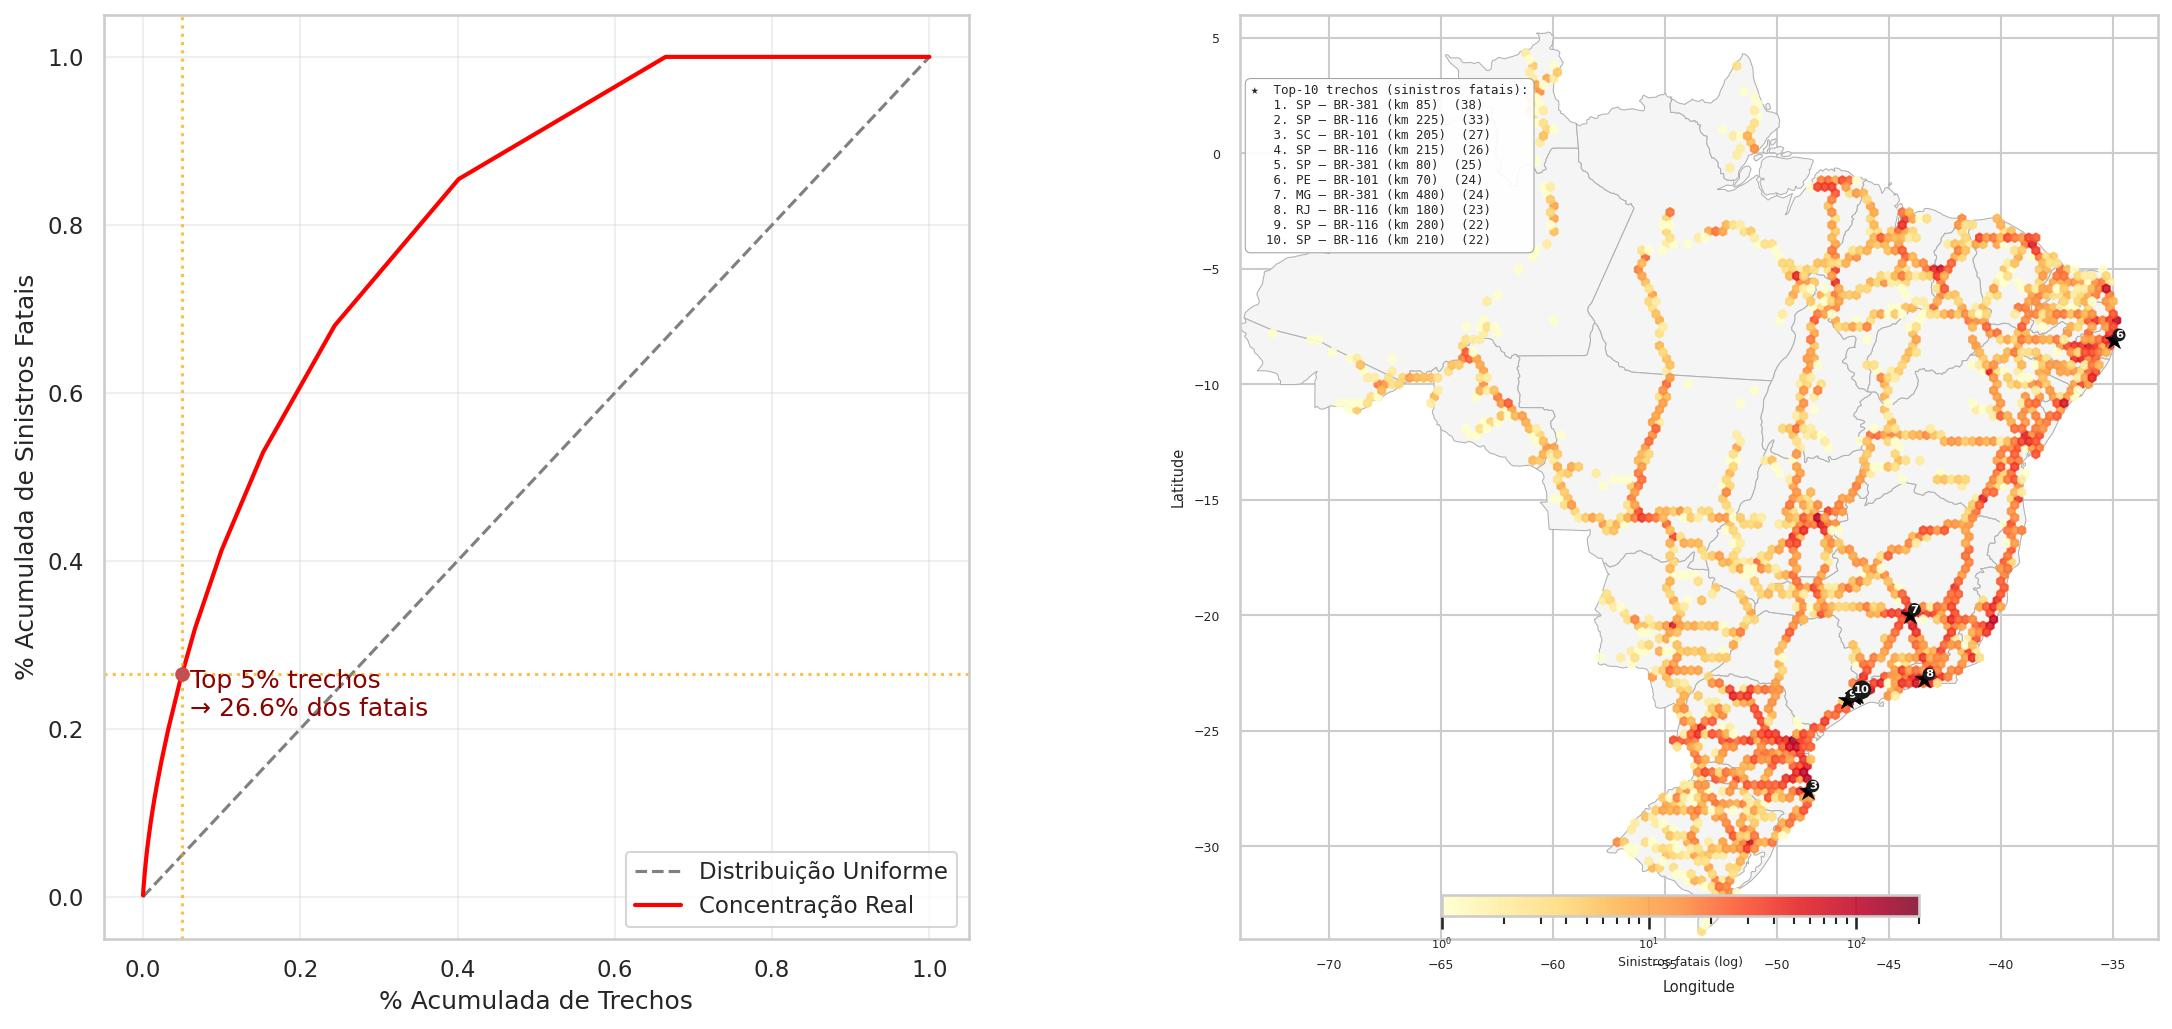
\includegraphics[width=\textwidth]{../figures/fig3.jpg}
\caption{Curva de Lorenz espacial (faixas de 5 km) e mapa de calor hexagonal dos sinistros fatais nas rodovias federais (2022--2026), em escala logarítmica. As estrelas numeradas indicam os dez trechos de 5 km com maior número absoluto de fatalidades; a legenda no canto superior esquerdo lista os identificadores completos.}
\label{fig:lorenz_espacial}
\end{figure}

\subsubsection{H5 --- Heterogeneidade Regional}

A verificação de H5 avaliou a associação entre a severidade dos acidentes, as regiões brasileiras e a infraestrutura viária (tipo de pista). O teste qui-quadrado de independência confirmou que a gravidade dos sinistros difere significativamente entre as cinco regiões ($\chi^2 = 2023{,}65$; $p < 0{,}001$; $V = 0{,}082$). A análise de cruzamento de dados revela que a taxa de fatalidade em pistas simples (9,88\%) é mais do que o dobro da registrada em pistas duplas (4,71\%) e múltiplas (4,19\%). 

A letalidade regional acompanha diretamente a proporção de pista simples de cada malha: as regiões Norte (69,90\% de pista simples nos sinistros) e Nordeste (55,52\%) registraram as maiores taxas de fatalidade (11,02\% e 10,33\%, respectivamente). Em contraste, o Sudeste, com apenas 40,43\% de seus acidentes em pista simples, registrou uma taxa de fatalidade de 5,74\%. Os testes post-hoc pairwise com correção de Bonferroni ($k=10$) indicaram que as diferenças de letalidade entre as regiões são estatisticamente significativas ($p_{adj} < 0,05$), com exceção das comparações Sul--Sudeste ($p_{adj} = 0{,}182$) e Norte--Nordeste ($p_{adj} = 0{,}111$). Assim, \textbf{H5 é confirmada}, evidenciando que a precariedade da infraestrutura regional (predomínio de pistas simples) atua como um fator estrutural de agravamento da letalidade.

\begin{figure}[ht]
\centering
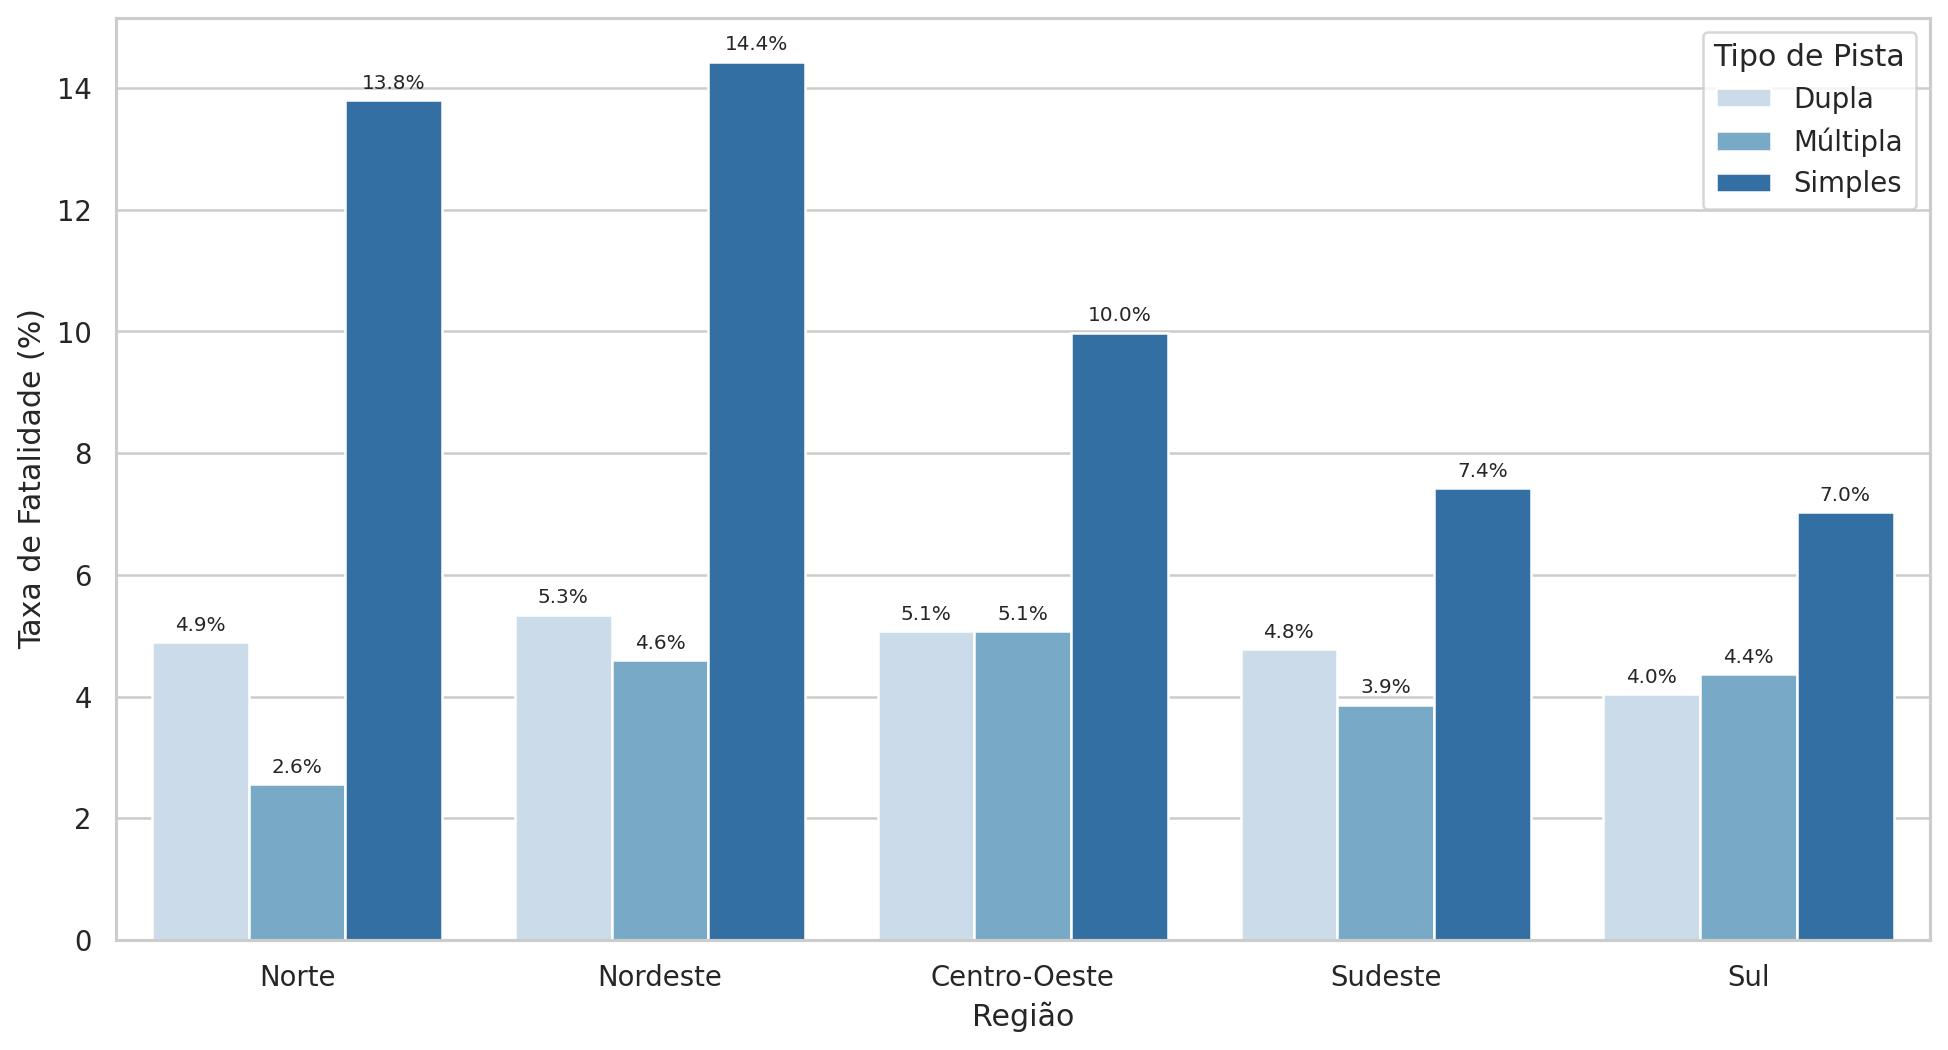
\includegraphics[width=0.9\textwidth]{../figures/fig4.jpg}
\caption{Taxa de fatalidade por região geográfica e tipo de pista. Regiões ordenadas da maior para a menor taxa agregada.}
\label{fig:regional_h5}
\end{figure}

% ============================================================
\section{Métodos e Métricas de Avaliação}
% ============================================================

Para avaliar as hipóteses formuladas, usamos abordagens complementares
de análise temporal, espacial e de associação bivariada. Como as
variáveis numéricas não seguem distribuição normal (assimetria
confirmada por QQ-plot em todas elas), optamos por testes não
paramétricos ao longo de toda a análise.

\subsection{Decomposição Temporal (STL)}
A análise temporal de H2 baseou-se na decomposição STL (\textit{Seasonal and Trend decomposition using Loess}) \cite{cleveland:1990}, parametrizada com período de 12 meses. O método separa a série mensal de sinistros em tendência, componente sazonal e resíduo. Para distinguir efeitos de volume e severidade, aplicamos a decomposição de forma independente sobre a série de volume de sinistros e sobre a série da proporção mensal de acidentes fatais. A métrica principal de avaliação foi a proporção da variância total explicada pela componente sazonal em cada série. Adicionalmente, aplicamos o teste $z$ de duas proporções para comparar a letalidade em recortes temporais específicos (fins de semana, feriados e férias).

\subsection{Concentração Espacial (Curva de Lorenz)}
Para testar a H4 (concentração espacial de fatalidades), calculamos a curva de Lorenz sobre as contagens de sinistros fatais discretizados nas faixas de 5 km. A curva quantifica a desigualdade na distribuição espacial sem assumir formas de agrupamentos predefinidos. Como métricas de concentração, extraímos a proporção de acidentes fatais acumulada nas faixas mais críticas (top 5\% e 10\%) e a fração mínima da malha necessária para responder por 50\% dos óbitos.

\subsection{Testes de Associação e Tamanho de Efeito}
Para as hipóteses H1, H3 e H5, usamos o teste qui-quadrado de independência de Pearson \cite{pearson:1900} com correção de viés para o V de Cramér \cite{bergsma:2013} como medida de tamanho de efeito de variáveis categóricas. Variáveis numéricas assimétricas foram avaliadas por teste de Kruskal-Wallis \cite{kruskal:1952} e tamanho de efeito $\varepsilon^2$. A força da associação de fatores de traçado ou meteorológicos com óbitos foi quantificada pela Razão de Chances (OR) com IC de 95\% e correção de Haldane-Anscombe. Comparações múltiplas pós-teste regional (post-hoc) foram corrigidas pelo método de Bonferroni.


% ============================================================
\section{Resultados e Discussão}
% ============================================================

Os testes estatísticos apontam para quatro frentes de ação.
Cada uma traduz um padrão dos dados em uma recomendação concreta
para PRF ou DNIT, com métrica de sucesso e prazo de avaliação.

\subsection{Insights Acionáveis}

\textbf{Infraestrutura — rotatórias como prioridade de obra.}
Trechos com rotatória apresentam chance de acidente fatal 71\%
menor que os demais (OR = 0{,}287; IC 95\% [0{,}246; 0{,}335]),
o maior efeito protetor entre todos os atributos de traçado analisados.
A geometria da rotatória reduz velocidade de impacto e ângulo de
colisão de forma estrutural. Recomendamos que o DNIT incorpore a
taxa de fatalidade por traçado como critério de priorização de obras,
com foco na conversão de interseções convencionais em rotatórias nos
trechos de maior concentração de ocorrências fatais. Após 24 meses,
o sucesso pode ser avaliado pela variação na taxa de fatalidade nos
trechos modificados, acompanhada pelo volume total de sinistros.
A intervenção será bem-sucedida se a taxa cair ao menos 30\% em
relação à linha de base pré-obra.

\textbf{Operações — efetivo concentrado nos fins de semana.}
Os dados mostram que fins de semana registram proporção fatal de
8,32\%, contra 6,62\% nos dias úteis (RR = 1,256; $p < 0{,}001$).
A decomposição STL confirma que esse efeito é de perfil de risco,
não de volume: a sazonalidade da gravidade (67,1\% da variância)
é independente da sazonalidade do volume de ocorrências (38,2\%).
Recomendamos que a PRF redistribua parte das operações de dias
úteis para o período de sexta a domingo, priorizando os trechos
do top-10 de fatalidade. O resultado pode ser monitorado mensalmente
pela proporção fatal nos fins de semana e será considerado positivo
se essa proporção convergir para a dos dias úteis em 12 meses.

\textbf{Fiscalização seletiva — trechos críticos identificados.}
Percebemos que 13,9\% da malha rodoviária federal concentra 50\%
de todos os sinistros fatais do período. Os eixos BR-381 (SP),
BR-116 (SP e RJ) e BR-101 (PE e SC) dominam o ranking de
faixas críticas de 5 km. Isso indica que a pulverização de
recursos ao longo de toda a malha é menos eficiente do que
a concentração nos trechos identificados. Recomendamos que
a PRF e o DNIT adotem o mapeamento de faixas críticas como
instrumento de planejamento operacional e de investimento em
infraestrutura. Após dois anos de atuação direcionada, o
sucesso pode ser avaliado pela redução na contagem de fatais
nos trechos priorizados em comparação com o período de base.

\textbf{Planejamento Viário — duplicação de eixos críticos regionais.}
Percebemos que as regiões Norte e Nordeste concentram as maiores taxas de fatalidade (11,02\% e 10,33\%) devido ao predomínio de pistas simples em seus sinistros (69,9\% e 55,5\%). Isso sugere que a gravidade regional não é meramente comportamental, mas condicionada pela infraestrutura viária de pista única. Por isso, recomendamos que o DNIT priorize obras de duplicação nos trechos críticos das rodovias BR-101 (Nordeste) e BR-316/010 (Norte/Nordeste), integrando o planejamento de expansão com o mapeamento de faixas críticas da PRF. A decisão foi sustentada pelo teste de qui-quadrado de severidade regional ($\chi^2 = 2023,65$; $p < 0,001$) e pelo contraste de letalidade pista simples vs. dupla (9,88\% vs 4,71\%). Após 36 meses do início das intervenções, o sucesso pode ser avaliado pela redução na taxa de fatalidade por trecho modificado. A ação será considerada bem-sucedida se a taxa de fatalidade nas rodovias duplicadas sofrer redução de pelo menos 40\% em relação à linha de base.


% ============================================================
\section{Conclusão}
% ============================================================

Este trabalho analisou 300.086 registros de sinistros em rodovias
federais brasileiras (2022--2026), percorrendo limpeza de dados,
engenharia de \textit{features}, análise exploratória bivariada e
verificação de cinco hipóteses por meio de testes estatísticos,
decomposição temporal e análise de concentração espacial. O tipo de
acidente revelou-se o preditor individual mais relevante para a
gravidade (V de Cramér = 0{,}344); entre os atributos de traçado,
rotatórias apresentam o maior efeito protetor (OR = 0{,}287), enquanto
pontes e declives concentram maior risco de fatalidade.

Os resultados desafiam algumas intuições operacionais. Causas
comportamentais são mais letais de dia do que à noite, o que sugere
redistribuir as blitzes de sobriedade para o período diurno. Fins de
semana e feriados elevam o risco, mas férias não, indicando que o
problema é comportamental, não de volume. A chuva não agrava a
gravidade; pelo contrário, os motoristas parecem compensar o risco
reduzindo a velocidade. O espaço é desigual: 13,9\% da malha
concentra metade das mortes. E a infraestrutura explica a desigualdade
regional: pistas simples mais que dobram a letalidade.

A principal limitação é a ausência de dados de volume de tráfego
por trecho. Sem eles, as taxas refletem contagens absolutas de
ocorrências, não exposição por veículo-km rodado. A base PRF é
construída a partir de boletins de atendimento, o que implica
subnotificação em regiões com cobertura operacional limitada,
especialmente no interior do Norte e do Nordeste. Por fim, os dados
de 2026 cobrem apenas uma fração do ano, o que pode distorcer
componentes sazonais se não for controlado explicitamente.

Como trabalhos futuros, recomenda-se incorporar dados de volume
veicular do DNIT para calcular taxas de exposição, explorar modelos
\textit{ensemble} para capturar interações entre variáveis, e
desenvolver um sistema de alerta por trecho que combine os
indicadores de concentração espacial com as variáveis temporais
identificadas neste trabalho.


% ============================================================
\bibliographystyle{sbc}
\bibliography{referencias}
% ============================================================

\end{document}
